\subsection{Cross Database Performance Evaluation}

From the within database experiment, we can clearly get a conclusion that the RITL loss function can increase the performance compare to the STTL loss function, and the RFNet is better than the DeConvRFNet, EfficientNetV2-S, and FKNet. Meanwhile, the FKNet performance is the worst one. In this section, we will compare these models' performance on the cross database experiment. For these cross database experiment, it can get the generalization ability of neural network, because these data can be regard as unseen data. 

As for the cross database experiment, I firstly pre-trained our models on the Finger Knuckle Images Database V1, and then fine-tuned models on the Finger Knuckle Images Database V3 (with deformation). In the next step, we use our models to test all the finger knuckle of the Hand Dorsal Images Database and the Tsinghua Finger Vein and Finger Dorsal Texture Database (THU-FVFDT3) \cite{thufvfdt3}. Although the THU-FVFDT3 database can offer two-session samples with interval several seconds, but strictly speaking, it is not two-session database. Therefore, I just use the training set of the database (THU-FVFDT-FDT3\_Train) as our evaluation dataset.

\subsubsection{Hand Dorsal Images Database}

\textbf{Index Finger Knuckle and Middle Finger Knuckle}

% \begin{figure}[ht!]
% 	\centering
% 	\begin{subfigure}[b]{0.45\linewidth}
% 		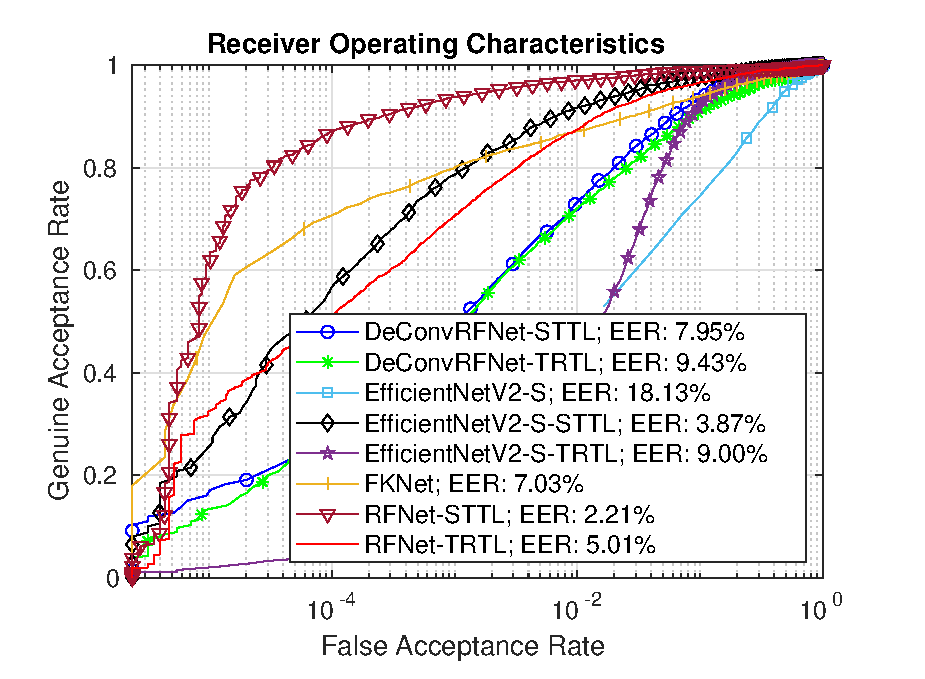
\includegraphics[width=\linewidth]{Figures/crosshd-roc_compare_new.eps}
% 		\caption{}
% 	\end{subfigure}
%     \begin{subfigure}[b]{0.45\linewidth}
% 		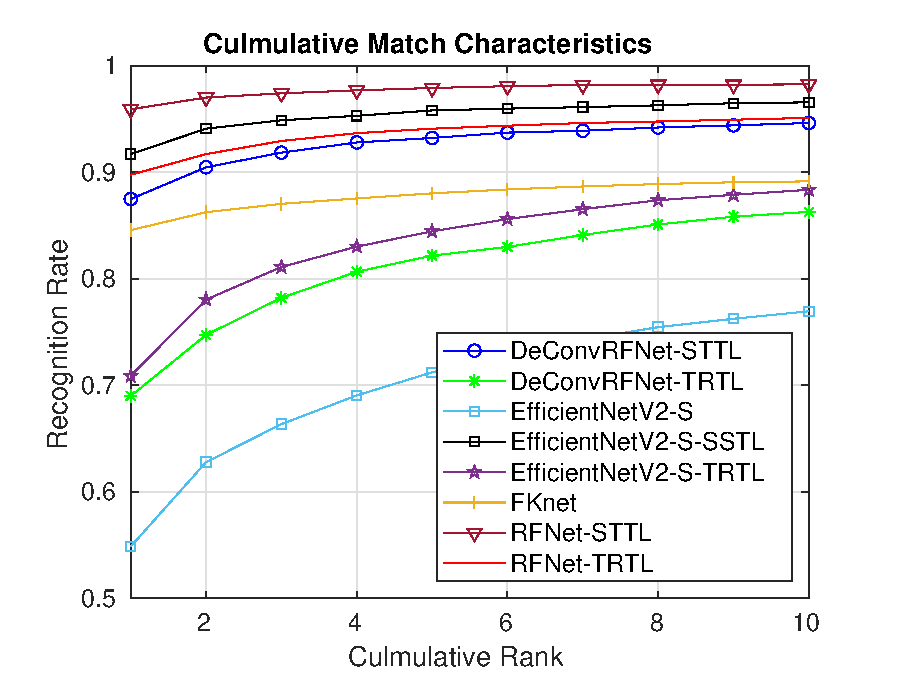
\includegraphics[width=\linewidth]{Figures/crosshd-cmc_compare_new.eps}
% 		\caption{}
% 	\end{subfigure}
% 	\caption{Comparative ROC (a) and corresponding CMC (b) for one-session of the index finger knuckle on the contactless hand dorsal image database \cite{ContactlessHnadDorsaldb}.}
% 	\label{crosshd-index-one-session}
% \end{figure}

% \begin{figure}[ht!]
% 	\centering
% 	\begin{subfigure}[b]{0.45\linewidth}
% 		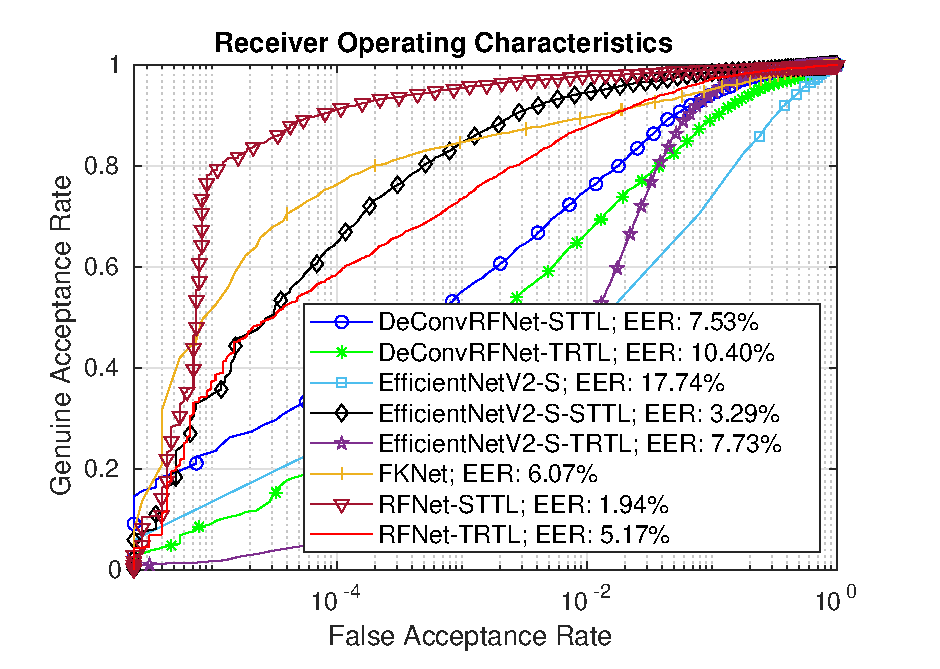
\includegraphics[width=\linewidth]{Figures/crosshd-middle-roc_compare_new.eps}
% 		\caption{}
% 	\end{subfigure}
%     \begin{subfigure}[b]{0.45\linewidth}
% 		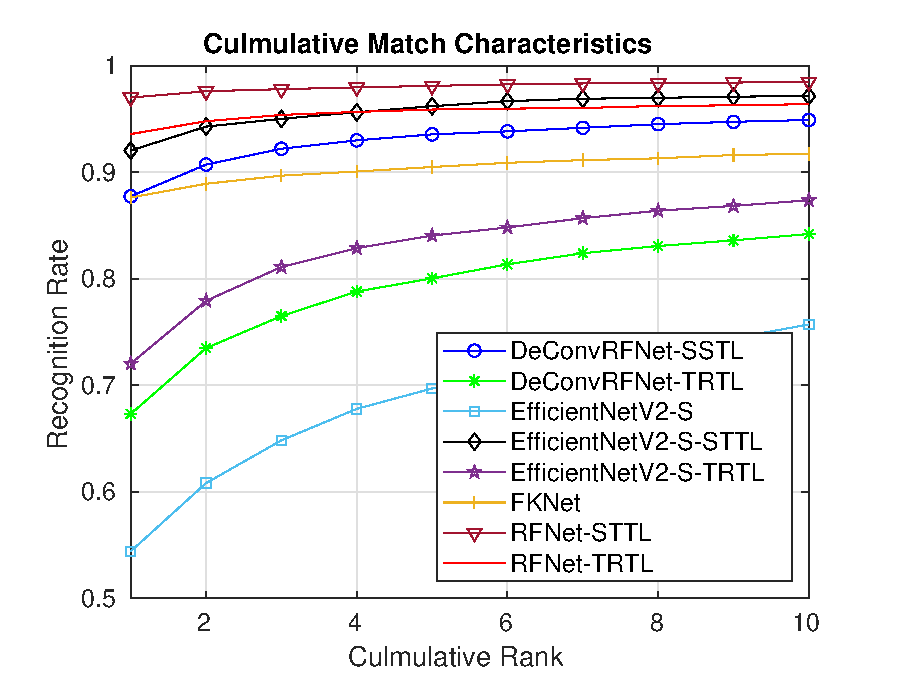
\includegraphics[width=\linewidth]{Figures/crosshd-middle-cmc_compare_new.eps}
% 		\caption{}
% 	\end{subfigure}
% 	\caption{Comparative ROC (a) and corresponding CMC (b) for one-session of the middle finger knuckle on the contactless hand dorsal image database \cite{ContactlessHnadDorsaldb}.}
% 	\label{crosshd-middle-one-session}
% \end{figure}

\begin{figure}[ht!]
	\centering
	\begin{subfigure}[b]{0.45\linewidth}
		\includegraphics[width=\linewidth]{Figures/cross-hd-index-fkv3(yolov5)-105-221/roc_compare_new.eps}
		\caption{}
	\end{subfigure}
    \begin{subfigure}[b]{0.45\linewidth}
		\includegraphics[width=\linewidth]{Figures/cross-hd-index-fkv3(yolov5)-105-221/cmc_compare_new.eps}
		\caption{}
	\end{subfigure}
	\caption{Comparative ROC (a) and corresponding CMC (b) for one-session of the index finger knuckle on the contactless hand dorsal image database \cite{ContactlessHnadDorsaldb}.}
	\label{crosshd-index-one-session}
\end{figure}

The database totally has 712 subjects, and each subject has 5 samples of hand dorsal image. Therefore, it will have $712*5=3560$ genuine matching scores and $712*711*5 = 2531160$ imposter matching scores for index and middle finger knuckle. Figure \ref{crosshd-index-one-session} is the performance result on the index finger.From Figure \ref{crosshd-index-one-session}, all models' cross database performance is similar on the database regardless which finger. We should also notice that STTL is better than RITL on the cross database experiment, while within database, the RITL is better than STTL. It shows that the generalization ability of RITL is not better than STTL to some extent. However, the RFNet-STTL outperform the rest models depend on the ROC and CMC. Even better than FKNet and EfficientNetV2-S, both of them are classification models.



\subsubsection{Tsinghua Finger Vein and Finger Dorsal Texture Database}
\begin{figure}[ht!]
	\centering
	\begin{subfigure}[b]{0.45\linewidth}
		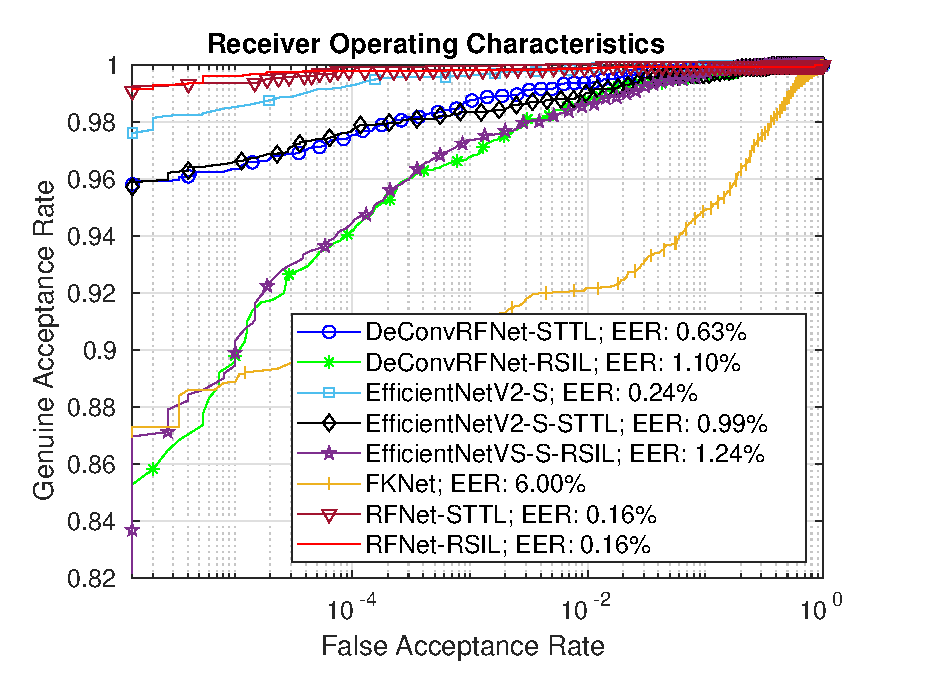
\includegraphics[width=\linewidth]{Figures/crossthu-roc_compare_new.eps}
		\caption{}
	\end{subfigure}
    \begin{subfigure}[b]{0.45\linewidth}
		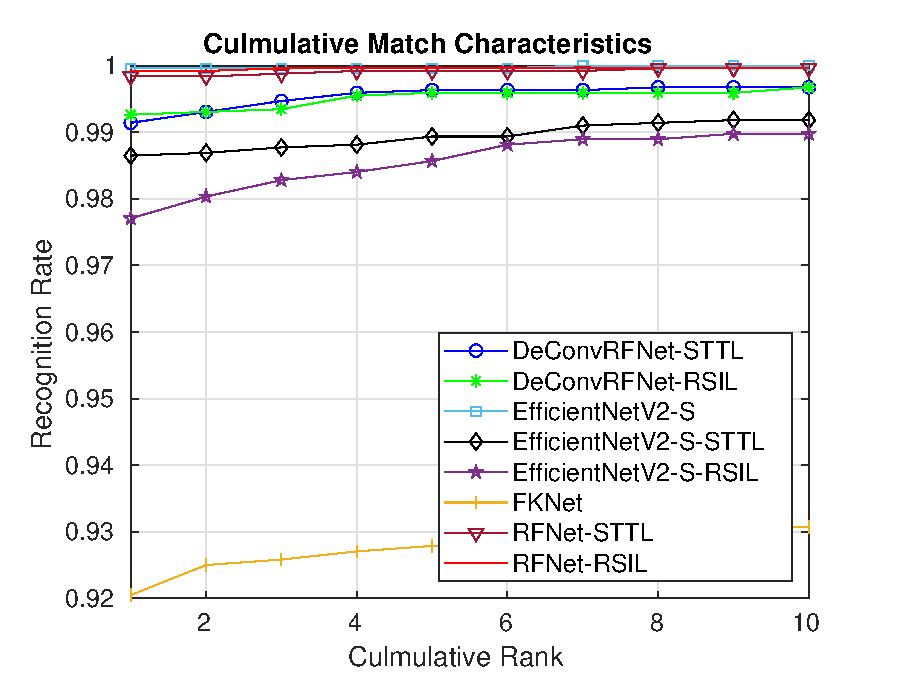
\includegraphics[width=\linewidth]{Figures/crossthu-cmc_compare_new.eps}
		\caption{}
	\end{subfigure}
	\caption{Comparative ROC (a) and corresponding CMC (b) for one-session of the finger dorsal texture images \cite{thufvfdt3}.}
	\label{crossthu-one-session}
\end{figure}

The database \cite{thufvfdt3} has 610 subjects, and each subject can offer 4 samples. From the finger dorsal texture images, we can use our YOLOv5-CSL model to segment finger knuckle images as our testing set. Then as the cross database experiment, it will have $610*4=2440$ genuine matching scores and $610*609*4=1485960$ imposter matching scores. In this database, all models can get very high matching performance from the Figure \ref{crossthu-one-session}, even the worst FKNet can arrive at $6.00\%$ EER on the database. The RFNet with RITL and STTL get the same accuracy, in terms of the CMC, the recognition rate almost arrive at $100\%$.
